\begin{document}
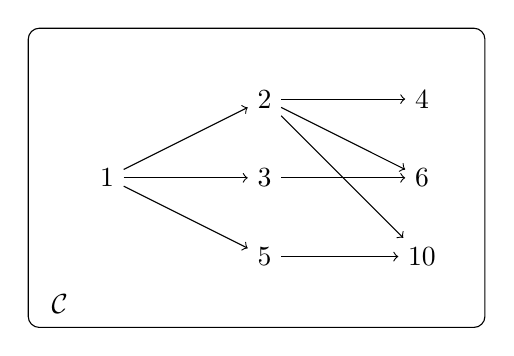
\begin{tikzpicture}
  \draw[rounded corners] (-1,-0.9) rectangle (4.8,2.9);
  \node at (-0.6,-0.6) {$\mathcal{C}$};
  \node (1) at (0,1) {$1$};
  \node (2) at (2,2) {$2$};
  \node (3) at (2,1) {$3$};
  \node (5) at (2,0) {$5$};
  \node (4) at (4,2) {$4$};
  \node (6) at (4,1) {$6$};
  \node (10) at (4,0) {$10$};
  \draw[->] (1) -- (2);
  \draw[->] (1) -- (3);
  \draw[->] (1) -- (5);
  \draw[->] (2) -- (4);
  \draw[->] (2) -- (6);
  \draw[->] (2) -- (10);
  \draw[->] (3) -- (6);
  \draw[->] (5) -- (10);
\end{tikzpicture}
\end{document}
